% Created by tikzDevice version 0.7.0 on 2014-07-26 02:56:07
% !TEX encoding = UTF-8 Unicode
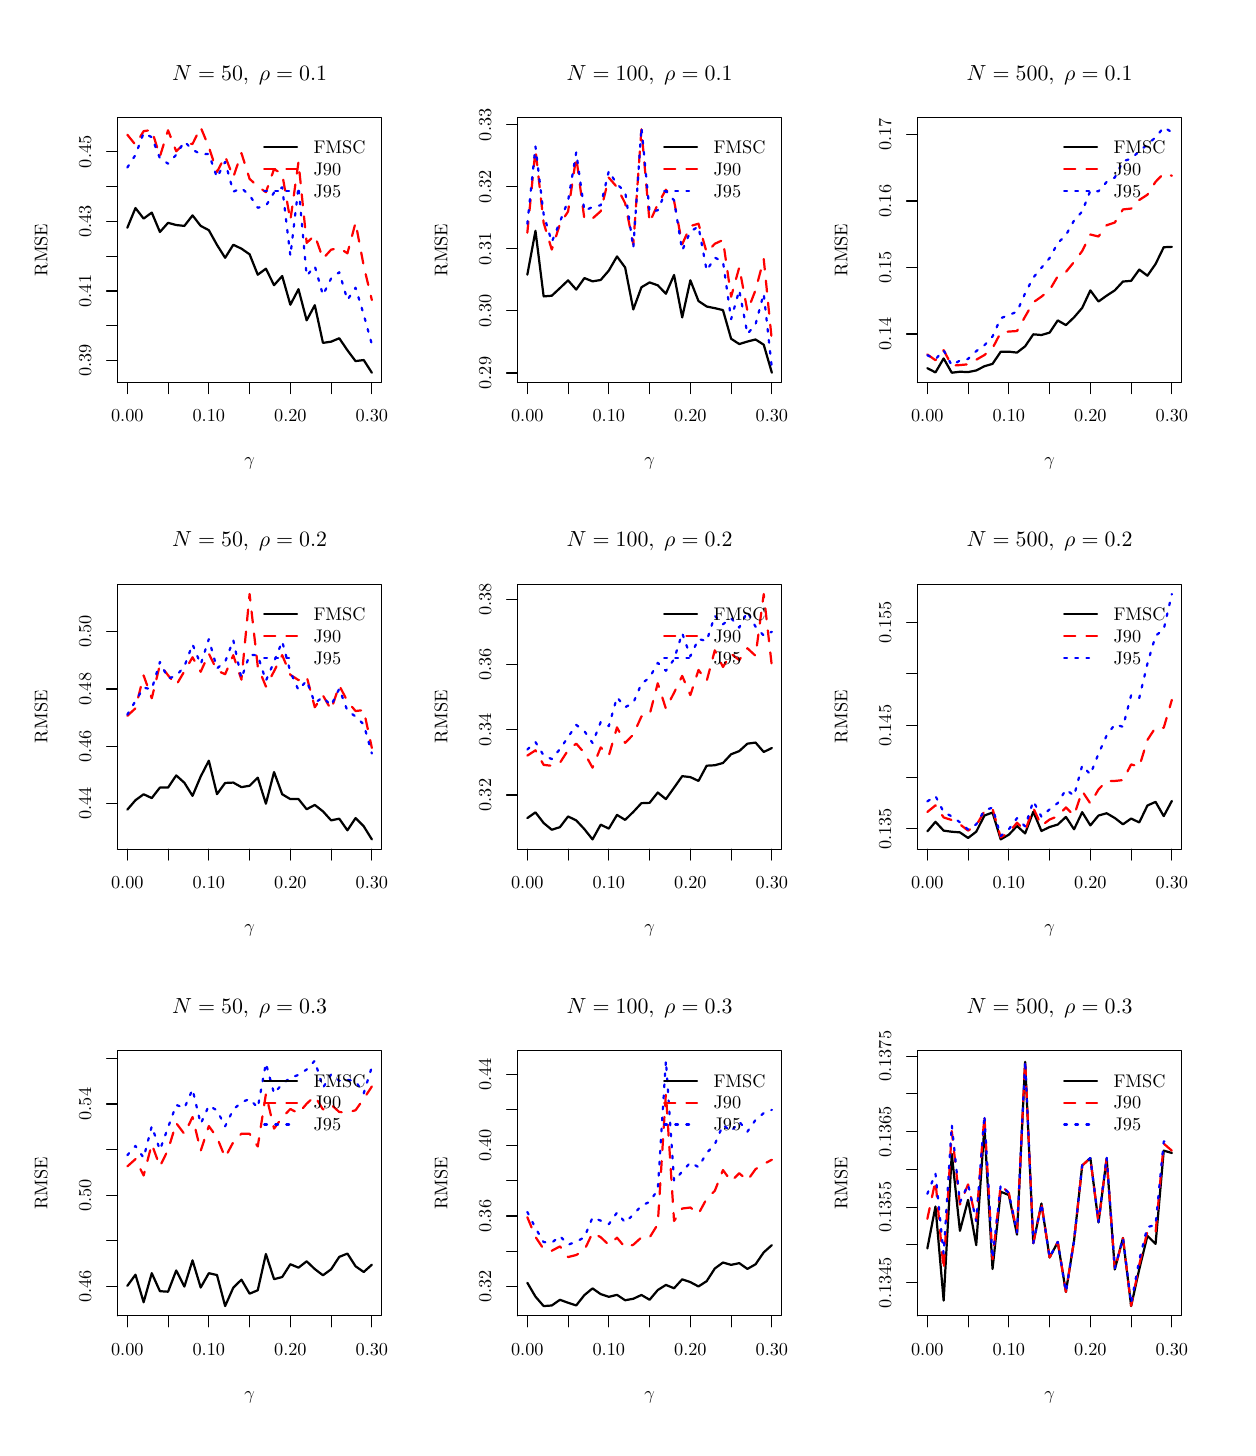
\begin{tikzpicture}[x=1pt,y=1pt]
\definecolor[named]{fillColor}{rgb}{1.00,1.00,1.00}
\path[use as bounding box,fill=fillColor,fill opacity=0.00] (0,0) rectangle (433.62,505.89);
\begin{scope}
\path[clip] ( 32.47,377.65) rectangle (127.91,473.42);
\definecolor[named]{drawColor}{rgb}{0.00,0.00,0.00}

\path[draw=drawColor,line width= 0.8pt,line join=round,line cap=round] ( 36.01,433.58) --
	( 38.95,440.71) --
	( 41.90,436.89) --
	( 44.84,439.07) --
	( 47.79,432.05) --
	( 50.73,435.37) --
	( 53.68,434.57) --
	( 56.63,434.25) --
	( 59.57,438.06) --
	( 62.52,434.26) --
	( 65.46,432.70) --
	( 68.41,427.40) --
	( 71.35,422.72) --
	( 74.30,427.44) --
	( 77.24,426.03) --
	( 80.19,423.99) --
	( 83.14,416.62) --
	( 86.08,418.79) --
	( 89.03,412.83) --
	( 91.97,416.14) --
	( 94.92,405.76) --
	( 97.86,411.37) --
	(100.81,400.12) --
	(103.75,405.60) --
	(106.70,391.98) --
	(109.65,392.42) --
	(112.59,393.66) --
	(115.54,389.32) --
	(118.48,385.40) --
	(121.43,385.79) --
	(124.37,381.20);
\end{scope}
\begin{scope}
\path[clip] (  0.00,  0.00) rectangle (433.62,505.89);
\definecolor[named]{drawColor}{rgb}{0.00,0.00,0.00}

\path[draw=drawColor,line width= 0.4pt,line join=round,line cap=round] ( 36.01,377.65) -- (124.37,377.65);

\path[draw=drawColor,line width= 0.4pt,line join=round,line cap=round] ( 36.01,377.65) -- ( 36.01,373.69);

\path[draw=drawColor,line width= 0.4pt,line join=round,line cap=round] ( 50.73,377.65) -- ( 50.73,373.69);

\path[draw=drawColor,line width= 0.4pt,line join=round,line cap=round] ( 65.46,377.65) -- ( 65.46,373.69);

\path[draw=drawColor,line width= 0.4pt,line join=round,line cap=round] ( 80.19,377.65) -- ( 80.19,373.69);

\path[draw=drawColor,line width= 0.4pt,line join=round,line cap=round] ( 94.92,377.65) -- ( 94.92,373.69);

\path[draw=drawColor,line width= 0.4pt,line join=round,line cap=round] (109.65,377.65) -- (109.65,373.69);

\path[draw=drawColor,line width= 0.4pt,line join=round,line cap=round] (124.37,377.65) -- (124.37,373.69);

\node[text=drawColor,anchor=base,inner sep=0pt, outer sep=0pt, scale=  0.66] at ( 36.01,363.40) {0.00};

\node[text=drawColor,anchor=base,inner sep=0pt, outer sep=0pt, scale=  0.66] at ( 65.46,363.40) {0.10};

\node[text=drawColor,anchor=base,inner sep=0pt, outer sep=0pt, scale=  0.66] at ( 94.92,363.40) {0.20};

\node[text=drawColor,anchor=base,inner sep=0pt, outer sep=0pt, scale=  0.66] at (124.37,363.40) {0.30};

\path[draw=drawColor,line width= 0.4pt,line join=round,line cap=round] ( 32.47,385.59) -- ( 32.47,461.01);

\path[draw=drawColor,line width= 0.4pt,line join=round,line cap=round] ( 32.47,385.59) -- ( 28.51,385.59);

\path[draw=drawColor,line width= 0.4pt,line join=round,line cap=round] ( 32.47,398.16) -- ( 28.51,398.16);

\path[draw=drawColor,line width= 0.4pt,line join=round,line cap=round] ( 32.47,410.73) -- ( 28.51,410.73);

\path[draw=drawColor,line width= 0.4pt,line join=round,line cap=round] ( 32.47,423.30) -- ( 28.51,423.30);

\path[draw=drawColor,line width= 0.4pt,line join=round,line cap=round] ( 32.47,435.87) -- ( 28.51,435.87);

\path[draw=drawColor,line width= 0.4pt,line join=round,line cap=round] ( 32.47,448.44) -- ( 28.51,448.44);

\path[draw=drawColor,line width= 0.4pt,line join=round,line cap=round] ( 32.47,461.01) -- ( 28.51,461.01);

\node[text=drawColor,rotate= 90.00,anchor=base,inner sep=0pt, outer sep=0pt, scale=  0.66] at ( 22.97,385.59) {0.39};

\node[text=drawColor,rotate= 90.00,anchor=base,inner sep=0pt, outer sep=0pt, scale=  0.66] at ( 22.97,410.73) {0.41};

\node[text=drawColor,rotate= 90.00,anchor=base,inner sep=0pt, outer sep=0pt, scale=  0.66] at ( 22.97,435.87) {0.43};

\node[text=drawColor,rotate= 90.00,anchor=base,inner sep=0pt, outer sep=0pt, scale=  0.66] at ( 22.97,461.01) {0.45};

\path[draw=drawColor,line width= 0.4pt,line join=round,line cap=round] ( 32.47,377.65) --
	(127.91,377.65) --
	(127.91,473.42) --
	( 32.47,473.42) --
	( 32.47,377.65);
\end{scope}
\begin{scope}
\path[clip] (  0.00,337.26) rectangle (144.54,505.89);
\definecolor[named]{drawColor}{rgb}{0.00,0.00,0.00}

\node[text=drawColor,anchor=base,inner sep=0pt, outer sep=0pt, scale=  0.79] at ( 80.19,486.92) {\bfseries $N=50, \;\rho=0.1$};

\node[text=drawColor,anchor=base,inner sep=0pt, outer sep=0pt, scale=  0.66] at ( 80.19,347.56) {$\gamma$};

\node[text=drawColor,rotate= 90.00,anchor=base,inner sep=0pt, outer sep=0pt, scale=  0.66] at (  7.13,425.53) {RMSE};
\end{scope}
\begin{scope}
\path[clip] ( 32.47,377.65) rectangle (127.91,473.42);
\definecolor[named]{drawColor}{rgb}{1.00,0.00,0.00}

\path[draw=drawColor,line width= 0.8pt,dash pattern=on 4pt off 4pt ,line join=round,line cap=round] ( 36.01,467.20) --
	( 38.95,463.56) --
	( 41.90,468.49) --
	( 44.84,468.92) --
	( 47.79,459.34) --
	( 50.73,468.81) --
	( 53.68,461.21) --
	( 56.63,464.11) --
	( 59.57,463.86) --
	( 62.52,469.87) --
	( 65.46,462.77) --
	( 68.41,453.73) --
	( 71.35,459.44) --
	( 74.30,451.84) --
	( 77.24,460.56) --
	( 80.19,451.25) --
	( 83.14,448.54) --
	( 86.08,446.43) --
	( 89.03,454.76) --
	( 91.97,453.04) --
	( 94.92,436.24) --
	( 97.86,457.35) --
	(100.81,428.11) --
	(103.75,430.87) --
	(106.70,422.42) --
	(109.65,425.67) --
	(112.59,426.28) --
	(115.54,424.35) --
	(118.48,435.44) --
	(121.43,419.81) --
	(124.37,407.46);
\definecolor[named]{drawColor}{rgb}{0.00,0.00,1.00}

\path[draw=drawColor,line width= 0.8pt,dash pattern=on 1pt off 3pt ,line join=round,line cap=round] ( 36.01,455.35) --
	( 38.95,459.89) --
	( 41.90,467.78) --
	( 44.84,466.31) --
	( 47.79,458.67) --
	( 50.73,456.74) --
	( 53.68,459.95) --
	( 56.63,464.75) --
	( 59.57,461.79) --
	( 62.52,460.19) --
	( 65.46,460.21) --
	( 68.41,451.75) --
	( 71.35,457.39) --
	( 74.30,446.61) --
	( 77.24,447.90) --
	( 80.19,445.32) --
	( 83.14,440.82) --
	( 86.08,441.46) --
	( 89.03,446.32) --
	( 91.97,448.21) --
	( 94.92,423.45) --
	( 97.86,448.42) --
	(100.81,416.21) --
	(103.75,419.71) --
	(106.70,409.27) --
	(109.65,415.26) --
	(112.59,417.50) --
	(115.54,407.49) --
	(118.48,411.91) --
	(121.43,402.20) --
	(124.37,391.45);
\definecolor[named]{drawColor}{rgb}{0.00,0.00,0.00}

\path[draw=drawColor,line width= 0.8pt,line join=round,line cap=round] ( 85.47,462.63) -- ( 97.35,462.63);
\definecolor[named]{drawColor}{rgb}{1.00,0.00,0.00}

\path[draw=drawColor,line width= 0.8pt,dash pattern=on 4pt off 4pt ,line join=round,line cap=round] ( 85.47,454.71) -- ( 97.35,454.71);
\definecolor[named]{drawColor}{rgb}{0.00,0.00,1.00}

\path[draw=drawColor,line width= 0.8pt,dash pattern=on 1pt off 3pt ,line join=round,line cap=round] ( 85.47,446.79) -- ( 97.35,446.79);
\definecolor[named]{drawColor}{rgb}{0.00,0.00,0.00}

\node[text=drawColor,anchor=base west,inner sep=0pt, outer sep=0pt, scale=  0.66] at (103.29,460.35) {FMSC};

\node[text=drawColor,anchor=base west,inner sep=0pt, outer sep=0pt, scale=  0.66] at (103.29,452.43) {J90};

\node[text=drawColor,anchor=base west,inner sep=0pt, outer sep=0pt, scale=  0.66] at (103.29,444.51) {J95};
\end{scope}
\begin{scope}
\path[clip] (177.01,377.65) rectangle (272.45,473.42);
\definecolor[named]{drawColor}{rgb}{0.00,0.00,0.00}

\path[draw=drawColor,line width= 0.8pt,line join=round,line cap=round] (180.55,416.63) --
	(183.49,432.48) --
	(186.44,408.78) --
	(189.38,409.02) --
	(192.33,411.77) --
	(195.27,414.58) --
	(198.22,411.24) --
	(201.17,415.40) --
	(204.11,414.22) --
	(207.06,414.71) --
	(210.00,418.12) --
	(212.95,423.22) --
	(215.89,419.23) --
	(218.84,404.07) --
	(221.78,412.08) --
	(224.73,413.83) --
	(227.68,412.79) --
	(230.62,409.74) --
	(233.57,416.53) --
	(236.51,401.18) --
	(239.46,414.59) --
	(242.40,407.10) --
	(245.35,405.13) --
	(248.29,404.53) --
	(251.24,403.83) --
	(254.19,393.47) --
	(257.13,391.56) --
	(260.08,392.47) --
	(263.02,393.21) --
	(265.97,391.32) --
	(268.91,381.20);
\end{scope}
\begin{scope}
\path[clip] (  0.00,  0.00) rectangle (433.62,505.89);
\definecolor[named]{drawColor}{rgb}{0.00,0.00,0.00}

\path[draw=drawColor,line width= 0.4pt,line join=round,line cap=round] (180.55,377.65) -- (268.91,377.65);

\path[draw=drawColor,line width= 0.4pt,line join=round,line cap=round] (180.55,377.65) -- (180.55,373.69);

\path[draw=drawColor,line width= 0.4pt,line join=round,line cap=round] (195.27,377.65) -- (195.27,373.69);

\path[draw=drawColor,line width= 0.4pt,line join=round,line cap=round] (210.00,377.65) -- (210.00,373.69);

\path[draw=drawColor,line width= 0.4pt,line join=round,line cap=round] (224.73,377.65) -- (224.73,373.69);

\path[draw=drawColor,line width= 0.4pt,line join=round,line cap=round] (239.46,377.65) -- (239.46,373.69);

\path[draw=drawColor,line width= 0.4pt,line join=round,line cap=round] (254.19,377.65) -- (254.19,373.69);

\path[draw=drawColor,line width= 0.4pt,line join=round,line cap=round] (268.91,377.65) -- (268.91,373.69);

\node[text=drawColor,anchor=base,inner sep=0pt, outer sep=0pt, scale=  0.66] at (180.55,363.40) {0.00};

\node[text=drawColor,anchor=base,inner sep=0pt, outer sep=0pt, scale=  0.66] at (210.00,363.40) {0.10};

\node[text=drawColor,anchor=base,inner sep=0pt, outer sep=0pt, scale=  0.66] at (239.46,363.40) {0.20};

\node[text=drawColor,anchor=base,inner sep=0pt, outer sep=0pt, scale=  0.66] at (268.91,363.40) {0.30};

\path[draw=drawColor,line width= 0.4pt,line join=round,line cap=round] (177.01,381.11) -- (177.01,470.77);

\path[draw=drawColor,line width= 0.4pt,line join=round,line cap=round] (177.01,381.11) -- (173.05,381.11);

\path[draw=drawColor,line width= 0.4pt,line join=round,line cap=round] (177.01,403.53) -- (173.05,403.53);

\path[draw=drawColor,line width= 0.4pt,line join=round,line cap=round] (177.01,425.94) -- (173.05,425.94);

\path[draw=drawColor,line width= 0.4pt,line join=round,line cap=round] (177.01,448.36) -- (173.05,448.36);

\path[draw=drawColor,line width= 0.4pt,line join=round,line cap=round] (177.01,470.77) -- (173.05,470.77);

\node[text=drawColor,rotate= 90.00,anchor=base,inner sep=0pt, outer sep=0pt, scale=  0.66] at (167.51,381.11) {0.29};

\node[text=drawColor,rotate= 90.00,anchor=base,inner sep=0pt, outer sep=0pt, scale=  0.66] at (167.51,403.53) {0.30};

\node[text=drawColor,rotate= 90.00,anchor=base,inner sep=0pt, outer sep=0pt, scale=  0.66] at (167.51,425.94) {0.31};

\node[text=drawColor,rotate= 90.00,anchor=base,inner sep=0pt, outer sep=0pt, scale=  0.66] at (167.51,448.36) {0.32};

\node[text=drawColor,rotate= 90.00,anchor=base,inner sep=0pt, outer sep=0pt, scale=  0.66] at (167.51,470.77) {0.33};

\path[draw=drawColor,line width= 0.4pt,line join=round,line cap=round] (177.01,377.65) --
	(272.45,377.65) --
	(272.45,473.42) --
	(177.01,473.42) --
	(177.01,377.65);
\end{scope}
\begin{scope}
\path[clip] (144.54,337.26) rectangle (289.08,505.89);
\definecolor[named]{drawColor}{rgb}{0.00,0.00,0.00}

\node[text=drawColor,anchor=base,inner sep=0pt, outer sep=0pt, scale=  0.79] at (224.73,486.92) {\bfseries $N=100, \;\rho=0.1$};

\node[text=drawColor,anchor=base,inner sep=0pt, outer sep=0pt, scale=  0.66] at (224.73,347.56) {$\gamma$};

\node[text=drawColor,rotate= 90.00,anchor=base,inner sep=0pt, outer sep=0pt, scale=  0.66] at (151.67,425.53) {RMSE};
\end{scope}
\begin{scope}
\path[clip] (177.01,377.65) rectangle (272.45,473.42);
\definecolor[named]{drawColor}{rgb}{1.00,0.00,0.00}

\path[draw=drawColor,line width= 0.8pt,dash pattern=on 4pt off 4pt ,line join=round,line cap=round] (180.55,431.80) --
	(183.49,461.89) --
	(186.44,435.34) --
	(189.38,425.70) --
	(192.33,434.91) --
	(195.27,439.46) --
	(198.22,459.19) --
	(201.17,436.70) --
	(204.11,436.93) --
	(207.06,439.56) --
	(210.00,451.68) --
	(212.95,448.26) --
	(215.89,442.44) --
	(218.84,427.57) --
	(221.78,469.18) --
	(224.73,435.48) --
	(227.68,442.09) --
	(230.62,447.33) --
	(233.57,443.33) --
	(236.51,427.62) --
	(239.46,434.20) --
	(242.40,435.05) --
	(245.35,424.65) --
	(248.29,427.79) --
	(251.24,429.16) --
	(254.19,408.67) --
	(257.13,419.29) --
	(260.08,403.49) --
	(263.02,411.08) --
	(265.97,422.25) --
	(268.91,392.80);
\definecolor[named]{drawColor}{rgb}{0.00,0.00,1.00}

\path[draw=drawColor,line width= 0.8pt,dash pattern=on 1pt off 3pt ,line join=round,line cap=round] (180.55,435.01) --
	(183.49,462.96) --
	(186.44,438.44) --
	(189.38,428.42) --
	(192.33,435.75) --
	(195.27,443.32) --
	(198.22,460.83) --
	(201.17,439.69) --
	(204.11,441.11) --
	(207.06,441.71) --
	(210.00,454.08) --
	(212.95,449.25) --
	(215.89,446.73) --
	(218.84,426.35) --
	(221.78,469.87) --
	(224.73,439.32) --
	(227.68,439.90) --
	(230.62,446.86) --
	(233.57,443.49) --
	(236.51,425.37) --
	(239.46,432.23) --
	(242.40,434.02) --
	(245.35,418.10) --
	(248.29,422.77) --
	(251.24,421.41) --
	(254.19,400.55) --
	(257.13,411.04) --
	(260.08,395.21) --
	(263.02,398.72) --
	(265.97,409.79) --
	(268.91,382.91);
\definecolor[named]{drawColor}{rgb}{0.00,0.00,0.00}

\path[draw=drawColor,line width= 0.8pt,line join=round,line cap=round] (230.01,462.63) -- (241.89,462.63);
\definecolor[named]{drawColor}{rgb}{1.00,0.00,0.00}

\path[draw=drawColor,line width= 0.8pt,dash pattern=on 4pt off 4pt ,line join=round,line cap=round] (230.01,454.71) -- (241.89,454.71);
\definecolor[named]{drawColor}{rgb}{0.00,0.00,1.00}

\path[draw=drawColor,line width= 0.8pt,dash pattern=on 1pt off 3pt ,line join=round,line cap=round] (230.01,446.79) -- (241.89,446.79);
\definecolor[named]{drawColor}{rgb}{0.00,0.00,0.00}

\node[text=drawColor,anchor=base west,inner sep=0pt, outer sep=0pt, scale=  0.66] at (247.83,460.35) {FMSC};

\node[text=drawColor,anchor=base west,inner sep=0pt, outer sep=0pt, scale=  0.66] at (247.83,452.43) {J90};

\node[text=drawColor,anchor=base west,inner sep=0pt, outer sep=0pt, scale=  0.66] at (247.83,444.51) {J95};
\end{scope}
\begin{scope}
\path[clip] (321.55,377.65) rectangle (416.99,473.42);
\definecolor[named]{drawColor}{rgb}{0.00,0.00,0.00}

\path[draw=drawColor,line width= 0.8pt,line join=round,line cap=round] (325.09,382.85) --
	(328.03,381.31) --
	(330.98,386.36) --
	(333.92,381.20) --
	(336.87,381.56) --
	(339.81,381.43) --
	(342.76,382.02) --
	(345.71,383.54) --
	(348.65,384.40) --
	(351.60,388.77) --
	(354.54,388.81) --
	(357.49,388.47) --
	(360.43,390.75) --
	(363.38,395.08) --
	(366.32,394.83) --
	(369.27,395.69) --
	(372.22,400.11) --
	(375.16,398.41) --
	(378.11,401.22) --
	(381.05,404.63) --
	(384.00,410.95) --
	(386.94,406.93) --
	(389.89,409.05) --
	(392.83,410.97) --
	(395.78,414.15) --
	(398.73,414.40) --
	(401.67,418.47) --
	(404.62,416.26) --
	(407.56,420.49) --
	(410.51,426.55) --
	(413.45,426.68);
\end{scope}
\begin{scope}
\path[clip] (  0.00,  0.00) rectangle (433.62,505.89);
\definecolor[named]{drawColor}{rgb}{0.00,0.00,0.00}

\path[draw=drawColor,line width= 0.4pt,line join=round,line cap=round] (325.09,377.65) -- (413.45,377.65);

\path[draw=drawColor,line width= 0.4pt,line join=round,line cap=round] (325.09,377.65) -- (325.09,373.69);

\path[draw=drawColor,line width= 0.4pt,line join=round,line cap=round] (339.81,377.65) -- (339.81,373.69);

\path[draw=drawColor,line width= 0.4pt,line join=round,line cap=round] (354.54,377.65) -- (354.54,373.69);

\path[draw=drawColor,line width= 0.4pt,line join=round,line cap=round] (369.27,377.65) -- (369.27,373.69);

\path[draw=drawColor,line width= 0.4pt,line join=round,line cap=round] (384.00,377.65) -- (384.00,373.69);

\path[draw=drawColor,line width= 0.4pt,line join=round,line cap=round] (398.73,377.65) -- (398.73,373.69);

\path[draw=drawColor,line width= 0.4pt,line join=round,line cap=round] (413.45,377.65) -- (413.45,373.69);

\node[text=drawColor,anchor=base,inner sep=0pt, outer sep=0pt, scale=  0.66] at (325.09,363.40) {0.00};

\node[text=drawColor,anchor=base,inner sep=0pt, outer sep=0pt, scale=  0.66] at (354.54,363.40) {0.10};

\node[text=drawColor,anchor=base,inner sep=0pt, outer sep=0pt, scale=  0.66] at (384.00,363.40) {0.20};

\node[text=drawColor,anchor=base,inner sep=0pt, outer sep=0pt, scale=  0.66] at (413.45,363.40) {0.30};

\path[draw=drawColor,line width= 0.4pt,line join=round,line cap=round] (321.55,395.21) -- (321.55,467.29);

\path[draw=drawColor,line width= 0.4pt,line join=round,line cap=round] (321.55,395.21) -- (317.59,395.21);

\path[draw=drawColor,line width= 0.4pt,line join=round,line cap=round] (321.55,419.23) -- (317.59,419.23);

\path[draw=drawColor,line width= 0.4pt,line join=round,line cap=round] (321.55,443.26) -- (317.59,443.26);

\path[draw=drawColor,line width= 0.4pt,line join=round,line cap=round] (321.55,467.29) -- (317.59,467.29);

\node[text=drawColor,rotate= 90.00,anchor=base,inner sep=0pt, outer sep=0pt, scale=  0.66] at (312.05,395.21) {0.14};

\node[text=drawColor,rotate= 90.00,anchor=base,inner sep=0pt, outer sep=0pt, scale=  0.66] at (312.05,419.23) {0.15};

\node[text=drawColor,rotate= 90.00,anchor=base,inner sep=0pt, outer sep=0pt, scale=  0.66] at (312.05,443.26) {0.16};

\node[text=drawColor,rotate= 90.00,anchor=base,inner sep=0pt, outer sep=0pt, scale=  0.66] at (312.05,467.29) {0.17};

\path[draw=drawColor,line width= 0.4pt,line join=round,line cap=round] (321.55,377.65) --
	(416.99,377.65) --
	(416.99,473.42) --
	(321.55,473.42) --
	(321.55,377.65);
\end{scope}
\begin{scope}
\path[clip] (289.08,337.26) rectangle (433.62,505.89);
\definecolor[named]{drawColor}{rgb}{0.00,0.00,0.00}

\node[text=drawColor,anchor=base,inner sep=0pt, outer sep=0pt, scale=  0.79] at (369.27,486.92) {\bfseries $N=500, \;\rho=0.1$};

\node[text=drawColor,anchor=base,inner sep=0pt, outer sep=0pt, scale=  0.66] at (369.27,347.56) {$\gamma$};

\node[text=drawColor,rotate= 90.00,anchor=base,inner sep=0pt, outer sep=0pt, scale=  0.66] at (296.21,425.53) {RMSE};
\end{scope}
\begin{scope}
\path[clip] (321.55,377.65) rectangle (416.99,473.42);
\definecolor[named]{drawColor}{rgb}{1.00,0.00,0.00}

\path[draw=drawColor,line width= 0.8pt,dash pattern=on 4pt off 4pt ,line join=round,line cap=round] (325.09,387.81) --
	(328.03,385.72) --
	(330.98,389.36) --
	(333.92,383.78) --
	(336.87,383.96) --
	(339.81,384.25) --
	(342.76,385.89) --
	(345.71,387.59) --
	(348.65,390.06) --
	(351.60,395.70) --
	(354.54,396.08) --
	(357.49,396.26) --
	(360.43,401.50) --
	(363.38,406.63) --
	(366.32,408.69) --
	(369.27,411.05) --
	(372.22,416.09) --
	(375.16,417.61) --
	(378.11,421.24) --
	(381.05,425.19) --
	(384.00,431.15) --
	(386.94,430.42) --
	(389.89,434.50) --
	(392.83,435.49) --
	(395.78,440.21) --
	(398.73,440.52) --
	(401.67,443.62) --
	(404.62,445.52) --
	(407.56,450.20) --
	(410.51,453.22) --
	(413.45,452.39);
\definecolor[named]{drawColor}{rgb}{0.00,0.00,1.00}

\path[draw=drawColor,line width= 0.8pt,dash pattern=on 1pt off 3pt ,line join=round,line cap=round] (325.09,387.51) --
	(328.03,386.05) --
	(330.98,389.32) --
	(333.92,383.86) --
	(336.87,385.61) --
	(339.81,386.19) --
	(342.76,389.01) --
	(345.71,391.12) --
	(348.65,394.30) --
	(351.60,400.90) --
	(354.54,402.04) --
	(357.49,403.25) --
	(360.43,409.92) --
	(363.38,415.56) --
	(366.32,419.13) --
	(369.27,422.63) --
	(372.22,428.04) --
	(375.16,430.92) --
	(378.11,436.21) --
	(381.05,439.47) --
	(384.00,447.00) --
	(386.94,446.78) --
	(389.89,450.14) --
	(392.83,451.75) --
	(395.78,457.64) --
	(398.73,458.53) --
	(401.67,461.26) --
	(404.62,463.68) --
	(407.56,466.25) --
	(410.51,469.87) --
	(413.45,468.11);
\definecolor[named]{drawColor}{rgb}{0.00,0.00,0.00}

\path[draw=drawColor,line width= 0.8pt,line join=round,line cap=round] (374.55,462.63) -- (386.43,462.63);
\definecolor[named]{drawColor}{rgb}{1.00,0.00,0.00}

\path[draw=drawColor,line width= 0.8pt,dash pattern=on 4pt off 4pt ,line join=round,line cap=round] (374.55,454.71) -- (386.43,454.71);
\definecolor[named]{drawColor}{rgb}{0.00,0.00,1.00}

\path[draw=drawColor,line width= 0.8pt,dash pattern=on 1pt off 3pt ,line join=round,line cap=round] (374.55,446.79) -- (386.43,446.79);
\definecolor[named]{drawColor}{rgb}{0.00,0.00,0.00}

\node[text=drawColor,anchor=base west,inner sep=0pt, outer sep=0pt, scale=  0.66] at (392.37,460.35) {FMSC};

\node[text=drawColor,anchor=base west,inner sep=0pt, outer sep=0pt, scale=  0.66] at (392.37,452.43) {J90};

\node[text=drawColor,anchor=base west,inner sep=0pt, outer sep=0pt, scale=  0.66] at (392.37,444.51) {J95};
\end{scope}
\begin{scope}
\path[clip] ( 32.47,209.02) rectangle (127.91,304.79);
\definecolor[named]{drawColor}{rgb}{0.00,0.00,0.00}

\path[draw=drawColor,line width= 0.8pt,line join=round,line cap=round] ( 36.01,223.31) --
	( 38.95,226.73) --
	( 41.90,228.88) --
	( 44.84,227.51) --
	( 47.79,231.30) --
	( 50.73,231.31) --
	( 53.68,235.69) --
	( 56.63,233.03) --
	( 59.57,228.31) --
	( 62.52,235.30) --
	( 65.46,241.00) --
	( 68.41,228.91) --
	( 71.35,232.97) --
	( 74.30,233.10) --
	( 77.24,231.45) --
	( 80.19,231.96) --
	( 83.14,234.89) --
	( 86.08,225.47) --
	( 89.03,236.90) --
	( 91.97,228.88) --
	( 94.92,227.13) --
	( 97.86,227.16) --
	(100.81,223.47) --
	(103.75,225.02) --
	(106.70,222.71) --
	(109.65,219.45) --
	(112.59,220.05) --
	(115.54,215.85) --
	(118.48,220.27) --
	(121.43,217.31) --
	(124.37,212.57);
\end{scope}
\begin{scope}
\path[clip] (  0.00,  0.00) rectangle (433.62,505.89);
\definecolor[named]{drawColor}{rgb}{0.00,0.00,0.00}

\path[draw=drawColor,line width= 0.4pt,line join=round,line cap=round] ( 36.01,209.02) -- (124.37,209.02);

\path[draw=drawColor,line width= 0.4pt,line join=round,line cap=round] ( 36.01,209.02) -- ( 36.01,205.06);

\path[draw=drawColor,line width= 0.4pt,line join=round,line cap=round] ( 50.73,209.02) -- ( 50.73,205.06);

\path[draw=drawColor,line width= 0.4pt,line join=round,line cap=round] ( 65.46,209.02) -- ( 65.46,205.06);

\path[draw=drawColor,line width= 0.4pt,line join=round,line cap=round] ( 80.19,209.02) -- ( 80.19,205.06);

\path[draw=drawColor,line width= 0.4pt,line join=round,line cap=round] ( 94.92,209.02) -- ( 94.92,205.06);

\path[draw=drawColor,line width= 0.4pt,line join=round,line cap=round] (109.65,209.02) -- (109.65,205.06);

\path[draw=drawColor,line width= 0.4pt,line join=round,line cap=round] (124.37,209.02) -- (124.37,205.06);

\node[text=drawColor,anchor=base,inner sep=0pt, outer sep=0pt, scale=  0.66] at ( 36.01,194.77) {0.00};

\node[text=drawColor,anchor=base,inner sep=0pt, outer sep=0pt, scale=  0.66] at ( 65.46,194.77) {0.10};

\node[text=drawColor,anchor=base,inner sep=0pt, outer sep=0pt, scale=  0.66] at ( 94.92,194.77) {0.20};

\node[text=drawColor,anchor=base,inner sep=0pt, outer sep=0pt, scale=  0.66] at (124.37,194.77) {0.30};

\path[draw=drawColor,line width= 0.4pt,line join=round,line cap=round] ( 32.47,225.46) -- ( 32.47,287.66);

\path[draw=drawColor,line width= 0.4pt,line join=round,line cap=round] ( 32.47,225.46) -- ( 28.51,225.46);

\path[draw=drawColor,line width= 0.4pt,line join=round,line cap=round] ( 32.47,246.19) -- ( 28.51,246.19);

\path[draw=drawColor,line width= 0.4pt,line join=round,line cap=round] ( 32.47,266.92) -- ( 28.51,266.92);

\path[draw=drawColor,line width= 0.4pt,line join=round,line cap=round] ( 32.47,287.66) -- ( 28.51,287.66);

\node[text=drawColor,rotate= 90.00,anchor=base,inner sep=0pt, outer sep=0pt, scale=  0.66] at ( 22.97,225.46) {0.44};

\node[text=drawColor,rotate= 90.00,anchor=base,inner sep=0pt, outer sep=0pt, scale=  0.66] at ( 22.97,246.19) {0.46};

\node[text=drawColor,rotate= 90.00,anchor=base,inner sep=0pt, outer sep=0pt, scale=  0.66] at ( 22.97,266.92) {0.48};

\node[text=drawColor,rotate= 90.00,anchor=base,inner sep=0pt, outer sep=0pt, scale=  0.66] at ( 22.97,287.66) {0.50};

\path[draw=drawColor,line width= 0.4pt,line join=round,line cap=round] ( 32.47,209.02) --
	(127.91,209.02) --
	(127.91,304.79) --
	( 32.47,304.79) --
	( 32.47,209.02);
\end{scope}
\begin{scope}
\path[clip] (  0.00,168.63) rectangle (144.54,337.26);
\definecolor[named]{drawColor}{rgb}{0.00,0.00,0.00}

\node[text=drawColor,anchor=base,inner sep=0pt, outer sep=0pt, scale=  0.79] at ( 80.19,318.29) {\bfseries $N=50, \;\rho=0.2$};

\node[text=drawColor,anchor=base,inner sep=0pt, outer sep=0pt, scale=  0.66] at ( 80.19,178.93) {$\gamma$};

\node[text=drawColor,rotate= 90.00,anchor=base,inner sep=0pt, outer sep=0pt, scale=  0.66] at (  7.13,256.90) {RMSE};
\end{scope}
\begin{scope}
\path[clip] ( 32.47,209.02) rectangle (127.91,304.79);
\definecolor[named]{drawColor}{rgb}{1.00,0.00,0.00}

\path[draw=drawColor,line width= 0.8pt,dash pattern=on 4pt off 4pt ,line join=round,line cap=round] ( 36.01,257.21) --
	( 38.95,259.94) --
	( 41.90,271.80) --
	( 44.84,263.58) --
	( 47.79,275.69) --
	( 50.73,271.87) --
	( 53.68,268.33) --
	( 56.63,273.32) --
	( 59.57,278.38) --
	( 62.52,273.13) --
	( 65.46,279.71) --
	( 68.41,273.61) --
	( 71.35,272.26) --
	( 74.30,279.13) --
	( 77.24,270.29) --
	( 80.19,301.24) --
	( 83.14,275.06) --
	( 86.08,267.80) --
	( 89.03,273.33) --
	( 91.97,279.16) --
	( 94.92,272.05) --
	( 97.86,270.13) --
	(100.81,271.43) --
	(103.75,260.33) --
	(106.70,264.59) --
	(109.65,259.40) --
	(112.59,268.21) --
	(115.54,262.44) --
	(118.48,258.97) --
	(121.43,259.28) --
	(124.37,245.62);
\definecolor[named]{drawColor}{rgb}{0.00,0.00,1.00}

\path[draw=drawColor,line width= 0.8pt,dash pattern=on 1pt off 3pt ,line join=round,line cap=round] ( 36.01,257.64) --
	( 38.95,262.59) --
	( 41.90,267.38) --
	( 44.84,266.83) --
	( 47.79,276.71) --
	( 50.73,270.72) --
	( 53.68,271.63) --
	( 56.63,275.11) --
	( 59.57,283.05) --
	( 62.52,275.84) --
	( 65.46,284.91) --
	( 68.41,274.37) --
	( 71.35,276.73) --
	( 74.30,284.55) --
	( 77.24,270.76) --
	( 80.19,279.28) --
	( 83.14,279.09) --
	( 86.08,269.89) --
	( 89.03,276.77) --
	( 91.97,284.13) --
	( 94.92,273.09) --
	( 97.86,266.52) --
	(100.81,269.95) --
	(103.75,261.88) --
	(106.70,263.95) --
	(109.65,260.94) --
	(112.59,267.02) --
	(115.54,259.05) --
	(118.48,256.99) --
	(121.43,254.09) --
	(124.37,243.60);
\definecolor[named]{drawColor}{rgb}{0.00,0.00,0.00}

\path[draw=drawColor,line width= 0.8pt,line join=round,line cap=round] ( 85.47,294.00) -- ( 97.35,294.00);
\definecolor[named]{drawColor}{rgb}{1.00,0.00,0.00}

\path[draw=drawColor,line width= 0.8pt,dash pattern=on 4pt off 4pt ,line join=round,line cap=round] ( 85.47,286.08) -- ( 97.35,286.08);
\definecolor[named]{drawColor}{rgb}{0.00,0.00,1.00}

\path[draw=drawColor,line width= 0.8pt,dash pattern=on 1pt off 3pt ,line join=round,line cap=round] ( 85.47,278.16) -- ( 97.35,278.16);
\definecolor[named]{drawColor}{rgb}{0.00,0.00,0.00}

\node[text=drawColor,anchor=base west,inner sep=0pt, outer sep=0pt, scale=  0.66] at (103.29,291.72) {FMSC};

\node[text=drawColor,anchor=base west,inner sep=0pt, outer sep=0pt, scale=  0.66] at (103.29,283.80) {J90};

\node[text=drawColor,anchor=base west,inner sep=0pt, outer sep=0pt, scale=  0.66] at (103.29,275.88) {J95};
\end{scope}
\begin{scope}
\path[clip] (177.01,209.02) rectangle (272.45,304.79);
\definecolor[named]{drawColor}{rgb}{0.00,0.00,0.00}

\path[draw=drawColor,line width= 0.8pt,line join=round,line cap=round] (180.55,220.27) --
	(183.49,222.34) --
	(186.44,218.50) --
	(189.38,216.06) --
	(192.33,217.00) --
	(195.27,220.86) --
	(198.22,219.44) --
	(201.17,216.27) --
	(204.11,212.57) --
	(207.06,217.89) --
	(210.00,216.47) --
	(212.95,221.41) --
	(215.89,219.63) --
	(218.84,222.50) --
	(221.78,225.66) --
	(224.73,225.78) --
	(227.68,229.51) --
	(230.62,227.13) --
	(233.57,231.25) --
	(236.51,235.42) --
	(239.46,235.08) --
	(242.40,233.70) --
	(245.35,239.20) --
	(248.29,239.36) --
	(251.24,240.18) --
	(254.19,243.34) --
	(257.13,244.48) --
	(260.08,247.16) --
	(263.02,247.56) --
	(265.97,244.16) --
	(268.91,245.59);
\end{scope}
\begin{scope}
\path[clip] (  0.00,  0.00) rectangle (433.62,505.89);
\definecolor[named]{drawColor}{rgb}{0.00,0.00,0.00}

\path[draw=drawColor,line width= 0.4pt,line join=round,line cap=round] (180.55,209.02) -- (268.91,209.02);

\path[draw=drawColor,line width= 0.4pt,line join=round,line cap=round] (180.55,209.02) -- (180.55,205.06);

\path[draw=drawColor,line width= 0.4pt,line join=round,line cap=round] (195.27,209.02) -- (195.27,205.06);

\path[draw=drawColor,line width= 0.4pt,line join=round,line cap=round] (210.00,209.02) -- (210.00,205.06);

\path[draw=drawColor,line width= 0.4pt,line join=round,line cap=round] (224.73,209.02) -- (224.73,205.06);

\path[draw=drawColor,line width= 0.4pt,line join=round,line cap=round] (239.46,209.02) -- (239.46,205.06);

\path[draw=drawColor,line width= 0.4pt,line join=round,line cap=round] (254.19,209.02) -- (254.19,205.06);

\path[draw=drawColor,line width= 0.4pt,line join=round,line cap=round] (268.91,209.02) -- (268.91,205.06);

\node[text=drawColor,anchor=base,inner sep=0pt, outer sep=0pt, scale=  0.66] at (180.55,194.77) {0.00};

\node[text=drawColor,anchor=base,inner sep=0pt, outer sep=0pt, scale=  0.66] at (210.00,194.77) {0.10};

\node[text=drawColor,anchor=base,inner sep=0pt, outer sep=0pt, scale=  0.66] at (239.46,194.77) {0.20};

\node[text=drawColor,anchor=base,inner sep=0pt, outer sep=0pt, scale=  0.66] at (268.91,194.77) {0.30};

\path[draw=drawColor,line width= 0.4pt,line join=round,line cap=round] (177.01,228.62) -- (177.01,299.25);

\path[draw=drawColor,line width= 0.4pt,line join=round,line cap=round] (177.01,228.62) -- (173.05,228.62);

\path[draw=drawColor,line width= 0.4pt,line join=round,line cap=round] (177.01,252.16) -- (173.05,252.16);

\path[draw=drawColor,line width= 0.4pt,line join=round,line cap=round] (177.01,275.70) -- (173.05,275.70);

\path[draw=drawColor,line width= 0.4pt,line join=round,line cap=round] (177.01,299.25) -- (173.05,299.25);

\node[text=drawColor,rotate= 90.00,anchor=base,inner sep=0pt, outer sep=0pt, scale=  0.66] at (167.51,228.62) {0.32};

\node[text=drawColor,rotate= 90.00,anchor=base,inner sep=0pt, outer sep=0pt, scale=  0.66] at (167.51,252.16) {0.34};

\node[text=drawColor,rotate= 90.00,anchor=base,inner sep=0pt, outer sep=0pt, scale=  0.66] at (167.51,275.70) {0.36};

\node[text=drawColor,rotate= 90.00,anchor=base,inner sep=0pt, outer sep=0pt, scale=  0.66] at (167.51,299.25) {0.38};

\path[draw=drawColor,line width= 0.4pt,line join=round,line cap=round] (177.01,209.02) --
	(272.45,209.02) --
	(272.45,304.79) --
	(177.01,304.79) --
	(177.01,209.02);
\end{scope}
\begin{scope}
\path[clip] (144.54,168.63) rectangle (289.08,337.26);
\definecolor[named]{drawColor}{rgb}{0.00,0.00,0.00}

\node[text=drawColor,anchor=base,inner sep=0pt, outer sep=0pt, scale=  0.79] at (224.73,318.29) {\bfseries $N=100, \;\rho=0.2$};

\node[text=drawColor,anchor=base,inner sep=0pt, outer sep=0pt, scale=  0.66] at (224.73,178.93) {$\gamma$};

\node[text=drawColor,rotate= 90.00,anchor=base,inner sep=0pt, outer sep=0pt, scale=  0.66] at (151.67,256.90) {RMSE};
\end{scope}
\begin{scope}
\path[clip] (177.01,209.02) rectangle (272.45,304.79);
\definecolor[named]{drawColor}{rgb}{1.00,0.00,0.00}

\path[draw=drawColor,line width= 0.8pt,dash pattern=on 4pt off 4pt ,line join=round,line cap=round] (180.55,242.85) --
	(183.49,244.76) --
	(186.44,239.49) --
	(189.38,239.17) --
	(192.33,240.24) --
	(195.27,244.80) --
	(198.22,247.18) --
	(201.17,243.78) --
	(204.11,238.49) --
	(207.06,245.81) --
	(210.00,242.84) --
	(212.95,253.06) --
	(215.89,247.44) --
	(218.84,250.45) --
	(221.78,257.00) --
	(224.73,257.64) --
	(227.68,268.99) --
	(230.62,259.81) --
	(233.57,265.58) --
	(236.51,271.65) --
	(239.46,264.72) --
	(242.40,273.80) --
	(245.35,269.77) --
	(248.29,280.90) --
	(251.24,274.87) --
	(254.19,279.64) --
	(257.13,277.39) --
	(260.08,281.63) --
	(263.02,278.90) --
	(265.97,301.24) --
	(268.91,275.09);
\definecolor[named]{drawColor}{rgb}{0.00,0.00,1.00}

\path[draw=drawColor,line width= 0.8pt,dash pattern=on 1pt off 3pt ,line join=round,line cap=round] (180.55,245.05) --
	(183.49,247.74) --
	(186.44,242.89) --
	(189.38,241.61) --
	(192.33,245.22) --
	(195.27,249.52) --
	(198.22,253.94) --
	(201.17,251.69) --
	(204.11,247.43) --
	(207.06,254.93) --
	(210.00,253.52) --
	(212.95,263.93) --
	(215.89,260.33) --
	(218.84,261.91) --
	(221.78,268.83) --
	(224.73,271.03) --
	(227.68,276.37) --
	(230.62,273.51) --
	(233.57,277.65) --
	(236.51,287.09) --
	(239.46,278.74) --
	(242.40,284.96) --
	(245.35,284.27) --
	(248.29,293.40) --
	(251.24,290.29) --
	(254.19,292.52) --
	(257.13,289.11) --
	(260.08,294.84) --
	(263.02,289.41) --
	(265.97,286.22) --
	(268.91,287.59);
\definecolor[named]{drawColor}{rgb}{0.00,0.00,0.00}

\path[draw=drawColor,line width= 0.8pt,line join=round,line cap=round] (230.01,294.00) -- (241.89,294.00);
\definecolor[named]{drawColor}{rgb}{1.00,0.00,0.00}

\path[draw=drawColor,line width= 0.8pt,dash pattern=on 4pt off 4pt ,line join=round,line cap=round] (230.01,286.08) -- (241.89,286.08);
\definecolor[named]{drawColor}{rgb}{0.00,0.00,1.00}

\path[draw=drawColor,line width= 0.8pt,dash pattern=on 1pt off 3pt ,line join=round,line cap=round] (230.01,278.16) -- (241.89,278.16);
\definecolor[named]{drawColor}{rgb}{0.00,0.00,0.00}

\node[text=drawColor,anchor=base west,inner sep=0pt, outer sep=0pt, scale=  0.66] at (247.83,291.72) {FMSC};

\node[text=drawColor,anchor=base west,inner sep=0pt, outer sep=0pt, scale=  0.66] at (247.83,283.80) {J90};

\node[text=drawColor,anchor=base west,inner sep=0pt, outer sep=0pt, scale=  0.66] at (247.83,275.88) {J95};
\end{scope}
\begin{scope}
\path[clip] (321.55,209.02) rectangle (416.99,304.79);
\definecolor[named]{drawColor}{rgb}{0.00,0.00,0.00}

\path[draw=drawColor,line width= 0.8pt,line join=round,line cap=round] (325.09,215.46) --
	(328.03,218.92) --
	(330.98,215.74) --
	(333.92,215.33) --
	(336.87,215.11) --
	(339.81,213.09) --
	(342.76,215.34) --
	(345.71,221.20) --
	(348.65,222.28) --
	(351.60,212.57) --
	(354.54,214.27) --
	(357.49,217.40) --
	(360.43,214.72) --
	(363.38,222.58) --
	(366.32,215.61) --
	(369.27,217.04) --
	(372.22,217.94) --
	(375.16,220.69) --
	(378.11,216.23) --
	(381.05,222.41) --
	(384.00,217.63) --
	(386.94,221.19) --
	(389.89,222.02) --
	(392.83,220.30) --
	(395.78,218.02) --
	(398.73,220.11) --
	(401.67,218.69) --
	(404.62,224.81) --
	(407.56,226.13) --
	(410.51,220.98) --
	(413.45,226.48);
\end{scope}
\begin{scope}
\path[clip] (  0.00,  0.00) rectangle (433.62,505.89);
\definecolor[named]{drawColor}{rgb}{0.00,0.00,0.00}

\path[draw=drawColor,line width= 0.4pt,line join=round,line cap=round] (325.09,209.02) -- (413.45,209.02);

\path[draw=drawColor,line width= 0.4pt,line join=round,line cap=round] (325.09,209.02) -- (325.09,205.06);

\path[draw=drawColor,line width= 0.4pt,line join=round,line cap=round] (339.81,209.02) -- (339.81,205.06);

\path[draw=drawColor,line width= 0.4pt,line join=round,line cap=round] (354.54,209.02) -- (354.54,205.06);

\path[draw=drawColor,line width= 0.4pt,line join=round,line cap=round] (369.27,209.02) -- (369.27,205.06);

\path[draw=drawColor,line width= 0.4pt,line join=round,line cap=round] (384.00,209.02) -- (384.00,205.06);

\path[draw=drawColor,line width= 0.4pt,line join=round,line cap=round] (398.73,209.02) -- (398.73,205.06);

\path[draw=drawColor,line width= 0.4pt,line join=round,line cap=round] (413.45,209.02) -- (413.45,205.06);

\node[text=drawColor,anchor=base,inner sep=0pt, outer sep=0pt, scale=  0.66] at (325.09,194.77) {0.00};

\node[text=drawColor,anchor=base,inner sep=0pt, outer sep=0pt, scale=  0.66] at (354.54,194.77) {0.10};

\node[text=drawColor,anchor=base,inner sep=0pt, outer sep=0pt, scale=  0.66] at (384.00,194.77) {0.20};

\node[text=drawColor,anchor=base,inner sep=0pt, outer sep=0pt, scale=  0.66] at (413.45,194.77) {0.30};

\path[draw=drawColor,line width= 0.4pt,line join=round,line cap=round] (321.55,216.39) -- (321.55,291.04);

\path[draw=drawColor,line width= 0.4pt,line join=round,line cap=round] (321.55,216.39) -- (317.59,216.39);

\path[draw=drawColor,line width= 0.4pt,line join=round,line cap=round] (321.55,235.05) -- (317.59,235.05);

\path[draw=drawColor,line width= 0.4pt,line join=round,line cap=round] (321.55,253.71) -- (317.59,253.71);

\path[draw=drawColor,line width= 0.4pt,line join=round,line cap=round] (321.55,272.38) -- (317.59,272.38);

\path[draw=drawColor,line width= 0.4pt,line join=round,line cap=round] (321.55,291.04) -- (317.59,291.04);

\node[text=drawColor,rotate= 90.00,anchor=base,inner sep=0pt, outer sep=0pt, scale=  0.66] at (312.05,216.39) {0.135};

\node[text=drawColor,rotate= 90.00,anchor=base,inner sep=0pt, outer sep=0pt, scale=  0.66] at (312.05,253.71) {0.145};

\node[text=drawColor,rotate= 90.00,anchor=base,inner sep=0pt, outer sep=0pt, scale=  0.66] at (312.05,291.04) {0.155};

\path[draw=drawColor,line width= 0.4pt,line join=round,line cap=round] (321.55,209.02) --
	(416.99,209.02) --
	(416.99,304.79) --
	(321.55,304.79) --
	(321.55,209.02);
\end{scope}
\begin{scope}
\path[clip] (289.08,168.63) rectangle (433.62,337.26);
\definecolor[named]{drawColor}{rgb}{0.00,0.00,0.00}

\node[text=drawColor,anchor=base,inner sep=0pt, outer sep=0pt, scale=  0.79] at (369.27,318.29) {\bfseries $N=500, \;\rho=0.2$};

\node[text=drawColor,anchor=base,inner sep=0pt, outer sep=0pt, scale=  0.66] at (369.27,178.93) {$\gamma$};

\node[text=drawColor,rotate= 90.00,anchor=base,inner sep=0pt, outer sep=0pt, scale=  0.66] at (296.21,256.90) {RMSE};
\end{scope}
\begin{scope}
\path[clip] (321.55,209.02) rectangle (416.99,304.79);
\definecolor[named]{drawColor}{rgb}{1.00,0.00,0.00}

\path[draw=drawColor,line width= 0.8pt,dash pattern=on 4pt off 4pt ,line join=round,line cap=round] (325.09,222.48) --
	(328.03,224.87) --
	(330.98,220.52) --
	(333.92,219.55) --
	(336.87,218.00) --
	(339.81,215.75) --
	(342.76,217.62) --
	(345.71,222.70) --
	(348.65,223.62) --
	(351.60,213.29) --
	(354.54,215.04) --
	(357.49,218.60) --
	(360.43,215.64) --
	(363.38,223.91) --
	(366.32,217.52) --
	(369.27,219.75) --
	(372.22,220.95) --
	(375.16,224.12) --
	(378.11,221.22) --
	(381.05,230.01) --
	(384.00,225.52) --
	(386.94,230.61) --
	(389.89,233.70) --
	(392.83,233.69) --
	(395.78,234.00) --
	(398.73,239.66) --
	(401.67,238.84) --
	(404.62,248.52) --
	(407.56,253.00) --
	(410.51,252.91) --
	(413.45,263.00);
\definecolor[named]{drawColor}{rgb}{0.00,0.00,1.00}

\path[draw=drawColor,line width= 0.8pt,dash pattern=on 1pt off 3pt ,line join=round,line cap=round] (325.09,226.31) --
	(328.03,228.27) --
	(330.98,222.40) --
	(333.92,220.89) --
	(336.87,218.74) --
	(339.81,216.14) --
	(342.76,218.02) --
	(345.71,223.11) --
	(348.65,224.05) --
	(351.60,213.82) --
	(354.54,216.24) --
	(357.49,220.24) --
	(360.43,217.29) --
	(363.38,226.43) --
	(366.32,220.75) --
	(369.27,223.45) --
	(372.22,225.69) --
	(375.16,230.59) --
	(378.11,228.35) --
	(381.05,239.28) --
	(384.00,236.01) --
	(386.94,243.55) --
	(389.89,250.12) --
	(392.83,254.14) --
	(395.78,253.25) --
	(398.73,264.64) --
	(401.67,263.68) --
	(404.62,276.07) --
	(407.56,286.14) --
	(410.51,288.49) --
	(413.45,301.24);
\definecolor[named]{drawColor}{rgb}{0.00,0.00,0.00}

\path[draw=drawColor,line width= 0.8pt,line join=round,line cap=round] (374.55,294.00) -- (386.43,294.00);
\definecolor[named]{drawColor}{rgb}{1.00,0.00,0.00}

\path[draw=drawColor,line width= 0.8pt,dash pattern=on 4pt off 4pt ,line join=round,line cap=round] (374.55,286.08) -- (386.43,286.08);
\definecolor[named]{drawColor}{rgb}{0.00,0.00,1.00}

\path[draw=drawColor,line width= 0.8pt,dash pattern=on 1pt off 3pt ,line join=round,line cap=round] (374.55,278.16) -- (386.43,278.16);
\definecolor[named]{drawColor}{rgb}{0.00,0.00,0.00}

\node[text=drawColor,anchor=base west,inner sep=0pt, outer sep=0pt, scale=  0.66] at (392.37,291.72) {FMSC};

\node[text=drawColor,anchor=base west,inner sep=0pt, outer sep=0pt, scale=  0.66] at (392.37,283.80) {J90};

\node[text=drawColor,anchor=base west,inner sep=0pt, outer sep=0pt, scale=  0.66] at (392.37,275.88) {J95};
\end{scope}
\begin{scope}
\path[clip] ( 32.47, 40.39) rectangle (127.91,136.16);
\definecolor[named]{drawColor}{rgb}{0.00,0.00,0.00}

\path[draw=drawColor,line width= 0.8pt,line join=round,line cap=round] ( 36.01, 51.24) --
	( 38.95, 55.27) --
	( 41.90, 45.32) --
	( 44.84, 55.82) --
	( 47.79, 49.32) --
	( 50.73, 49.13) --
	( 53.68, 56.81) --
	( 56.63, 50.99) --
	( 59.57, 60.46) --
	( 62.52, 50.64) --
	( 65.46, 55.82) --
	( 68.41, 55.15) --
	( 71.35, 43.94) --
	( 74.30, 50.59) --
	( 77.24, 53.48) --
	( 80.19, 48.42) --
	( 83.14, 49.65) --
	( 86.08, 62.75) --
	( 89.03, 53.66) --
	( 91.97, 54.43) --
	( 94.92, 59.06) --
	( 97.86, 57.82) --
	(100.81, 60.11) --
	(103.75, 57.31) --
	(106.70, 55.07) --
	(109.65, 57.23) --
	(112.59, 61.72) --
	(115.54, 62.91) --
	(118.48, 58.32) --
	(121.43, 56.25) --
	(124.37, 58.89);
\end{scope}
\begin{scope}
\path[clip] (  0.00,  0.00) rectangle (433.62,505.89);
\definecolor[named]{drawColor}{rgb}{0.00,0.00,0.00}

\path[draw=drawColor,line width= 0.4pt,line join=round,line cap=round] ( 36.01, 40.39) -- (124.37, 40.39);

\path[draw=drawColor,line width= 0.4pt,line join=round,line cap=round] ( 36.01, 40.39) -- ( 36.01, 36.43);

\path[draw=drawColor,line width= 0.4pt,line join=round,line cap=round] ( 50.73, 40.39) -- ( 50.73, 36.43);

\path[draw=drawColor,line width= 0.4pt,line join=round,line cap=round] ( 65.46, 40.39) -- ( 65.46, 36.43);

\path[draw=drawColor,line width= 0.4pt,line join=round,line cap=round] ( 80.19, 40.39) -- ( 80.19, 36.43);

\path[draw=drawColor,line width= 0.4pt,line join=round,line cap=round] ( 94.92, 40.39) -- ( 94.92, 36.43);

\path[draw=drawColor,line width= 0.4pt,line join=round,line cap=round] (109.65, 40.39) -- (109.65, 36.43);

\path[draw=drawColor,line width= 0.4pt,line join=round,line cap=round] (124.37, 40.39) -- (124.37, 36.43);

\node[text=drawColor,anchor=base,inner sep=0pt, outer sep=0pt, scale=  0.66] at ( 36.01, 26.14) {0.00};

\node[text=drawColor,anchor=base,inner sep=0pt, outer sep=0pt, scale=  0.66] at ( 65.46, 26.14) {0.10};

\node[text=drawColor,anchor=base,inner sep=0pt, outer sep=0pt, scale=  0.66] at ( 94.92, 26.14) {0.20};

\node[text=drawColor,anchor=base,inner sep=0pt, outer sep=0pt, scale=  0.66] at (124.37, 26.14) {0.30};

\path[draw=drawColor,line width= 0.4pt,line join=round,line cap=round] ( 32.47, 51.10) -- ( 32.47,133.40);

\path[draw=drawColor,line width= 0.4pt,line join=round,line cap=round] ( 32.47, 51.10) -- ( 28.51, 51.10);

\path[draw=drawColor,line width= 0.4pt,line join=round,line cap=round] ( 32.47, 67.56) -- ( 28.51, 67.56);

\path[draw=drawColor,line width= 0.4pt,line join=round,line cap=round] ( 32.47, 84.02) -- ( 28.51, 84.02);

\path[draw=drawColor,line width= 0.4pt,line join=round,line cap=round] ( 32.47,100.48) -- ( 28.51,100.48);

\path[draw=drawColor,line width= 0.4pt,line join=round,line cap=round] ( 32.47,116.94) -- ( 28.51,116.94);

\path[draw=drawColor,line width= 0.4pt,line join=round,line cap=round] ( 32.47,133.40) -- ( 28.51,133.40);

\node[text=drawColor,rotate= 90.00,anchor=base,inner sep=0pt, outer sep=0pt, scale=  0.66] at ( 22.97, 51.10) {0.46};

\node[text=drawColor,rotate= 90.00,anchor=base,inner sep=0pt, outer sep=0pt, scale=  0.66] at ( 22.97, 84.02) {0.50};

\node[text=drawColor,rotate= 90.00,anchor=base,inner sep=0pt, outer sep=0pt, scale=  0.66] at ( 22.97,116.94) {0.54};

\path[draw=drawColor,line width= 0.4pt,line join=round,line cap=round] ( 32.47, 40.39) --
	(127.91, 40.39) --
	(127.91,136.16) --
	( 32.47,136.16) --
	( 32.47, 40.39);
\end{scope}
\begin{scope}
\path[clip] (  0.00,  0.00) rectangle (144.54,168.63);
\definecolor[named]{drawColor}{rgb}{0.00,0.00,0.00}

\node[text=drawColor,anchor=base,inner sep=0pt, outer sep=0pt, scale=  0.79] at ( 80.19,149.66) {\bfseries $N=50, \;\rho=0.3$};

\node[text=drawColor,anchor=base,inner sep=0pt, outer sep=0pt, scale=  0.66] at ( 80.19, 10.30) {$\gamma$};

\node[text=drawColor,rotate= 90.00,anchor=base,inner sep=0pt, outer sep=0pt, scale=  0.66] at (  7.13, 88.27) {RMSE};
\end{scope}
\begin{scope}
\path[clip] ( 32.47, 40.39) rectangle (127.91,136.16);
\definecolor[named]{drawColor}{rgb}{1.00,0.00,0.00}

\path[draw=drawColor,line width= 0.8pt,dash pattern=on 4pt off 4pt ,line join=round,line cap=round] ( 36.01, 94.40) --
	( 38.95, 97.04) --
	( 41.90, 91.11) --
	( 44.84,102.44) --
	( 47.79, 94.42) --
	( 50.73,100.41) --
	( 53.68,110.05) --
	( 56.63,106.13) --
	( 59.57,112.25) --
	( 62.52,100.05) --
	( 65.46,108.98) --
	( 68.41,104.86) --
	( 71.35, 97.66) --
	( 74.30,103.18) --
	( 77.24,106.25) --
	( 80.19,106.17) --
	( 83.14,101.61) --
	( 86.08,120.53) --
	( 89.03,108.05) --
	( 91.97,112.10) --
	( 94.92,115.15) --
	( 97.86,113.58) --
	(100.81,117.06) --
	(103.75,119.77) --
	(106.70,114.98) --
	(109.65,116.74) --
	(112.59,114.06) --
	(115.54,113.88) --
	(118.48,114.70) --
	(121.43,118.85) --
	(124.37,123.30);
\definecolor[named]{drawColor}{rgb}{0.00,0.00,1.00}

\path[draw=drawColor,line width= 0.8pt,dash pattern=on 1pt off 3pt ,line join=round,line cap=round] ( 36.01, 98.45) --
	( 38.95,101.79) --
	( 41.90, 97.53) --
	( 44.84,108.91) --
	( 47.79,100.37) --
	( 50.73,108.49) --
	( 53.68,116.63) --
	( 56.63,115.48) --
	( 59.57,122.25) --
	( 62.52,109.80) --
	( 65.46,116.36) --
	( 68.41,114.65) --
	( 71.35,108.91) --
	( 74.30,114.96) --
	( 77.24,117.56) --
	( 80.19,118.79) --
	( 83.14,115.61) --
	( 86.08,131.69) --
	( 89.03,120.76) --
	( 91.97,124.17) --
	( 94.92,126.47) --
	( 97.86,127.47) --
	(100.81,129.42) --
	(103.75,132.61) --
	(106.70,122.81) --
	(109.65,127.66) --
	(112.59,125.38) --
	(115.54,125.72) --
	(118.48,125.14) --
	(121.43,120.83) --
	(124.37,130.37);
\definecolor[named]{drawColor}{rgb}{0.00,0.00,0.00}

\path[draw=drawColor,line width= 0.8pt,line join=round,line cap=round] ( 85.47,125.37) -- ( 97.35,125.37);
\definecolor[named]{drawColor}{rgb}{1.00,0.00,0.00}

\path[draw=drawColor,line width= 0.8pt,dash pattern=on 4pt off 4pt ,line join=round,line cap=round] ( 85.47,117.45) -- ( 97.35,117.45);
\definecolor[named]{drawColor}{rgb}{0.00,0.00,1.00}

\path[draw=drawColor,line width= 0.8pt,dash pattern=on 1pt off 3pt ,line join=round,line cap=round] ( 85.47,109.53) -- ( 97.35,109.53);
\definecolor[named]{drawColor}{rgb}{0.00,0.00,0.00}

\node[text=drawColor,anchor=base west,inner sep=0pt, outer sep=0pt, scale=  0.66] at (103.29,123.09) {FMSC};

\node[text=drawColor,anchor=base west,inner sep=0pt, outer sep=0pt, scale=  0.66] at (103.29,115.17) {J90};

\node[text=drawColor,anchor=base west,inner sep=0pt, outer sep=0pt, scale=  0.66] at (103.29,107.25) {J95};
\end{scope}
\begin{scope}
\path[clip] (177.01, 40.39) rectangle (272.45,136.16);
\definecolor[named]{drawColor}{rgb}{0.00,0.00,0.00}

\path[draw=drawColor,line width= 0.8pt,line join=round,line cap=round] (180.55, 52.36) --
	(183.49, 47.35) --
	(186.44, 43.94) --
	(189.38, 44.15) --
	(192.33, 46.21) --
	(195.27, 45.14) --
	(198.22, 44.18) --
	(201.17, 47.91) --
	(204.11, 50.33) --
	(207.06, 48.25) --
	(210.00, 47.28) --
	(212.95, 48.00) --
	(215.89, 46.04) --
	(218.84, 46.58) --
	(221.78, 47.95) --
	(224.73, 46.22) --
	(227.68, 49.73) --
	(230.62, 51.58) --
	(233.57, 50.38) --
	(236.51, 53.61) --
	(239.46, 52.59) --
	(242.40, 51.03) --
	(245.35, 52.94) --
	(248.29, 57.51) --
	(251.24, 59.68) --
	(254.19, 58.83) --
	(257.13, 59.45) --
	(260.08, 57.36) --
	(263.02, 59.04) --
	(265.97, 63.35) --
	(268.91, 65.97);
\end{scope}
\begin{scope}
\path[clip] (  0.00,  0.00) rectangle (433.62,505.89);
\definecolor[named]{drawColor}{rgb}{0.00,0.00,0.00}

\path[draw=drawColor,line width= 0.4pt,line join=round,line cap=round] (180.55, 40.39) -- (268.91, 40.39);

\path[draw=drawColor,line width= 0.4pt,line join=round,line cap=round] (180.55, 40.39) -- (180.55, 36.43);

\path[draw=drawColor,line width= 0.4pt,line join=round,line cap=round] (195.27, 40.39) -- (195.27, 36.43);

\path[draw=drawColor,line width= 0.4pt,line join=round,line cap=round] (210.00, 40.39) -- (210.00, 36.43);

\path[draw=drawColor,line width= 0.4pt,line join=round,line cap=round] (224.73, 40.39) -- (224.73, 36.43);

\path[draw=drawColor,line width= 0.4pt,line join=round,line cap=round] (239.46, 40.39) -- (239.46, 36.43);

\path[draw=drawColor,line width= 0.4pt,line join=round,line cap=round] (254.19, 40.39) -- (254.19, 36.43);

\path[draw=drawColor,line width= 0.4pt,line join=round,line cap=round] (268.91, 40.39) -- (268.91, 36.43);

\node[text=drawColor,anchor=base,inner sep=0pt, outer sep=0pt, scale=  0.66] at (180.55, 26.14) {0.00};

\node[text=drawColor,anchor=base,inner sep=0pt, outer sep=0pt, scale=  0.66] at (210.00, 26.14) {0.10};

\node[text=drawColor,anchor=base,inner sep=0pt, outer sep=0pt, scale=  0.66] at (239.46, 26.14) {0.20};

\node[text=drawColor,anchor=base,inner sep=0pt, outer sep=0pt, scale=  0.66] at (268.91, 26.14) {0.30};

\path[draw=drawColor,line width= 0.4pt,line join=round,line cap=round] (177.01, 50.92) -- (177.01,127.59);

\path[draw=drawColor,line width= 0.4pt,line join=round,line cap=round] (177.01, 50.92) -- (173.05, 50.92);

\path[draw=drawColor,line width= 0.4pt,line join=round,line cap=round] (177.01, 63.70) -- (173.05, 63.70);

\path[draw=drawColor,line width= 0.4pt,line join=round,line cap=round] (177.01, 76.48) -- (173.05, 76.48);

\path[draw=drawColor,line width= 0.4pt,line join=round,line cap=round] (177.01, 89.26) -- (173.05, 89.26);

\path[draw=drawColor,line width= 0.4pt,line join=round,line cap=round] (177.01,102.03) -- (173.05,102.03);

\path[draw=drawColor,line width= 0.4pt,line join=round,line cap=round] (177.01,114.81) -- (173.05,114.81);

\path[draw=drawColor,line width= 0.4pt,line join=round,line cap=round] (177.01,127.59) -- (173.05,127.59);

\node[text=drawColor,rotate= 90.00,anchor=base,inner sep=0pt, outer sep=0pt, scale=  0.66] at (167.51, 50.92) {0.32};

\node[text=drawColor,rotate= 90.00,anchor=base,inner sep=0pt, outer sep=0pt, scale=  0.66] at (167.51, 76.48) {0.36};

\node[text=drawColor,rotate= 90.00,anchor=base,inner sep=0pt, outer sep=0pt, scale=  0.66] at (167.51,102.03) {0.40};

\node[text=drawColor,rotate= 90.00,anchor=base,inner sep=0pt, outer sep=0pt, scale=  0.66] at (167.51,127.59) {0.44};

\path[draw=drawColor,line width= 0.4pt,line join=round,line cap=round] (177.01, 40.39) --
	(272.45, 40.39) --
	(272.45,136.16) --
	(177.01,136.16) --
	(177.01, 40.39);
\end{scope}
\begin{scope}
\path[clip] (144.54,  0.00) rectangle (289.08,168.63);
\definecolor[named]{drawColor}{rgb}{0.00,0.00,0.00}

\node[text=drawColor,anchor=base,inner sep=0pt, outer sep=0pt, scale=  0.79] at (224.73,149.66) {\bfseries $N=100, \;\rho=0.3$};

\node[text=drawColor,anchor=base,inner sep=0pt, outer sep=0pt, scale=  0.66] at (224.73, 10.30) {$\gamma$};

\node[text=drawColor,rotate= 90.00,anchor=base,inner sep=0pt, outer sep=0pt, scale=  0.66] at (151.67, 88.27) {RMSE};
\end{scope}
\begin{scope}
\path[clip] (177.01, 40.39) rectangle (272.45,136.16);
\definecolor[named]{drawColor}{rgb}{1.00,0.00,0.00}

\path[draw=drawColor,line width= 0.8pt,dash pattern=on 4pt off 4pt ,line join=round,line cap=round] (180.55, 76.05) --
	(183.49, 68.94) --
	(186.44, 64.50) --
	(189.38, 63.93) --
	(192.33, 65.50) --
	(195.27, 61.66) --
	(198.22, 62.39) --
	(201.17, 64.15) --
	(204.11, 70.42) --
	(207.06, 68.82) --
	(210.00, 66.05) --
	(212.95, 68.64) --
	(215.89, 65.13) --
	(218.84, 66.10) --
	(221.78, 68.75) --
	(224.73, 68.72) --
	(227.68, 73.49) --
	(230.62,120.87) --
	(233.57, 74.68) --
	(236.51, 79.19) --
	(239.46, 79.55) --
	(242.40, 77.30) --
	(245.35, 82.73) --
	(248.29, 85.57) --
	(251.24, 93.09) --
	(254.19, 89.05) --
	(257.13, 91.93) --
	(260.08, 89.32) --
	(263.02, 93.42) --
	(265.97, 95.27) --
	(268.91, 96.81);
\definecolor[named]{drawColor}{rgb}{0.00,0.00,1.00}

\path[draw=drawColor,line width= 0.8pt,dash pattern=on 1pt off 3pt ,line join=round,line cap=round] (180.55, 77.95) --
	(183.49, 72.12) --
	(186.44, 67.08) --
	(189.38, 66.80) --
	(192.33, 69.27) --
	(195.27, 66.11) --
	(198.22, 67.18) --
	(201.17, 68.80) --
	(204.11, 75.95) --
	(207.06, 74.80) --
	(210.00, 73.52) --
	(212.95, 77.72) --
	(215.89, 74.14) --
	(218.84, 76.98) --
	(221.78, 80.22) --
	(224.73, 81.59) --
	(227.68, 85.96) --
	(230.62,132.61) --
	(233.57, 89.21) --
	(236.51, 92.55) --
	(239.46, 95.81) --
	(242.40, 94.15) --
	(245.35, 99.26) --
	(248.29,102.38) --
	(251.24,109.40) --
	(254.19,107.08) --
	(257.13,110.57) --
	(260.08,106.99) --
	(263.02,111.21) --
	(265.97,113.67) --
	(268.91,114.86);
\definecolor[named]{drawColor}{rgb}{0.00,0.00,0.00}

\path[draw=drawColor,line width= 0.8pt,line join=round,line cap=round] (230.01,125.37) -- (241.89,125.37);
\definecolor[named]{drawColor}{rgb}{1.00,0.00,0.00}

\path[draw=drawColor,line width= 0.8pt,dash pattern=on 4pt off 4pt ,line join=round,line cap=round] (230.01,117.45) -- (241.89,117.45);
\definecolor[named]{drawColor}{rgb}{0.00,0.00,1.00}

\path[draw=drawColor,line width= 0.8pt,dash pattern=on 1pt off 3pt ,line join=round,line cap=round] (230.01,109.53) -- (241.89,109.53);
\definecolor[named]{drawColor}{rgb}{0.00,0.00,0.00}

\node[text=drawColor,anchor=base west,inner sep=0pt, outer sep=0pt, scale=  0.66] at (247.83,123.09) {FMSC};

\node[text=drawColor,anchor=base west,inner sep=0pt, outer sep=0pt, scale=  0.66] at (247.83,115.17) {J90};

\node[text=drawColor,anchor=base west,inner sep=0pt, outer sep=0pt, scale=  0.66] at (247.83,107.25) {J95};
\end{scope}
\begin{scope}
\path[clip] (321.55, 40.39) rectangle (416.99,136.16);
\definecolor[named]{drawColor}{rgb}{0.00,0.00,0.00}

\path[draw=drawColor,line width= 0.8pt,line join=round,line cap=round] (325.09, 64.77) --
	(328.03, 79.92) --
	(330.98, 45.92) --
	(333.92, 98.93) --
	(336.87, 71.12) --
	(339.81, 82.31) --
	(342.76, 65.96) --
	(345.71,108.80) --
	(348.65, 57.33) --
	(351.60, 85.26) --
	(354.54, 84.07) --
	(357.49, 69.76) --
	(360.43,132.19) --
	(363.38, 66.62) --
	(366.32, 80.98) --
	(369.27, 61.48) --
	(372.22, 67.06) --
	(375.16, 49.05) --
	(378.11, 67.60) --
	(381.05, 94.73) --
	(384.00, 97.43) --
	(386.94, 74.13) --
	(389.89, 97.34) --
	(392.83, 57.18) --
	(395.78, 68.54) --
	(398.73, 43.94) --
	(401.67, 57.27) --
	(404.62, 69.31) --
	(407.56, 66.40) --
	(410.51,100.11) --
	(413.45, 99.26);
\end{scope}
\begin{scope}
\path[clip] (  0.00,  0.00) rectangle (433.62,505.89);
\definecolor[named]{drawColor}{rgb}{0.00,0.00,0.00}

\path[draw=drawColor,line width= 0.4pt,line join=round,line cap=round] (325.09, 40.39) -- (413.45, 40.39);

\path[draw=drawColor,line width= 0.4pt,line join=round,line cap=round] (325.09, 40.39) -- (325.09, 36.43);

\path[draw=drawColor,line width= 0.4pt,line join=round,line cap=round] (339.81, 40.39) -- (339.81, 36.43);

\path[draw=drawColor,line width= 0.4pt,line join=round,line cap=round] (354.54, 40.39) -- (354.54, 36.43);

\path[draw=drawColor,line width= 0.4pt,line join=round,line cap=round] (369.27, 40.39) -- (369.27, 36.43);

\path[draw=drawColor,line width= 0.4pt,line join=round,line cap=round] (384.00, 40.39) -- (384.00, 36.43);

\path[draw=drawColor,line width= 0.4pt,line join=round,line cap=round] (398.73, 40.39) -- (398.73, 36.43);

\path[draw=drawColor,line width= 0.4pt,line join=round,line cap=round] (413.45, 40.39) -- (413.45, 36.43);

\node[text=drawColor,anchor=base,inner sep=0pt, outer sep=0pt, scale=  0.66] at (325.09, 26.14) {0.00};

\node[text=drawColor,anchor=base,inner sep=0pt, outer sep=0pt, scale=  0.66] at (354.54, 26.14) {0.10};

\node[text=drawColor,anchor=base,inner sep=0pt, outer sep=0pt, scale=  0.66] at (384.00, 26.14) {0.20};

\node[text=drawColor,anchor=base,inner sep=0pt, outer sep=0pt, scale=  0.66] at (413.45, 26.14) {0.30};

\path[draw=drawColor,line width= 0.4pt,line join=round,line cap=round] (321.55, 52.41) -- (321.55,134.24);

\path[draw=drawColor,line width= 0.4pt,line join=round,line cap=round] (321.55, 52.41) -- (317.59, 52.41);

\path[draw=drawColor,line width= 0.4pt,line join=round,line cap=round] (321.55, 66.05) -- (317.59, 66.05);

\path[draw=drawColor,line width= 0.4pt,line join=round,line cap=round] (321.55, 79.69) -- (317.59, 79.69);

\path[draw=drawColor,line width= 0.4pt,line join=round,line cap=round] (321.55, 93.33) -- (317.59, 93.33);

\path[draw=drawColor,line width= 0.4pt,line join=round,line cap=round] (321.55,106.97) -- (317.59,106.97);

\path[draw=drawColor,line width= 0.4pt,line join=round,line cap=round] (321.55,120.61) -- (317.59,120.61);

\path[draw=drawColor,line width= 0.4pt,line join=round,line cap=round] (321.55,134.24) -- (317.59,134.24);

\node[text=drawColor,rotate= 90.00,anchor=base,inner sep=0pt, outer sep=0pt, scale=  0.66] at (312.05, 52.41) {0.1345};

\node[text=drawColor,rotate= 90.00,anchor=base,inner sep=0pt, outer sep=0pt, scale=  0.66] at (312.05, 79.69) {0.1355};

\node[text=drawColor,rotate= 90.00,anchor=base,inner sep=0pt, outer sep=0pt, scale=  0.66] at (312.05,106.97) {0.1365};

\node[text=drawColor,rotate= 90.00,anchor=base,inner sep=0pt, outer sep=0pt, scale=  0.66] at (312.05,134.24) {0.1375};

\path[draw=drawColor,line width= 0.4pt,line join=round,line cap=round] (321.55, 40.39) --
	(416.99, 40.39) --
	(416.99,136.16) --
	(321.55,136.16) --
	(321.55, 40.39);
\end{scope}
\begin{scope}
\path[clip] (289.08,  0.00) rectangle (433.62,168.63);
\definecolor[named]{drawColor}{rgb}{0.00,0.00,0.00}

\node[text=drawColor,anchor=base,inner sep=0pt, outer sep=0pt, scale=  0.79] at (369.27,149.66) {\bfseries $N=500, \;\rho=0.3$};

\node[text=drawColor,anchor=base,inner sep=0pt, outer sep=0pt, scale=  0.66] at (369.27, 10.30) {$\gamma$};

\node[text=drawColor,rotate= 90.00,anchor=base,inner sep=0pt, outer sep=0pt, scale=  0.66] at (296.21, 88.28) {RMSE};
\end{scope}
\begin{scope}
\path[clip] (321.55, 40.39) rectangle (416.99,136.16);
\definecolor[named]{drawColor}{rgb}{1.00,0.00,0.00}

\path[draw=drawColor,line width= 0.8pt,dash pattern=on 4pt off 4pt ,line join=round,line cap=round] (325.09, 75.45) --
	(328.03, 89.26) --
	(330.98, 57.01) --
	(333.92,107.20) --
	(336.87, 80.64) --
	(339.81, 87.92) --
	(342.76, 74.68) --
	(345.71,112.70) --
	(348.65, 60.84) --
	(351.60, 87.59) --
	(354.54, 84.83) --
	(357.49, 70.53) --
	(360.43,132.61) --
	(363.38, 66.72) --
	(366.32, 80.96) --
	(369.27, 61.55) --
	(372.22, 67.11) --
	(375.16, 49.07) --
	(378.11, 67.59) --
	(381.05, 94.73) --
	(384.00, 97.43) --
	(386.94, 74.13) --
	(389.89, 97.34) --
	(392.83, 57.18) --
	(395.78, 68.54) --
	(398.73, 44.03) --
	(401.67, 58.87) --
	(404.62, 70.92) --
	(407.56, 70.45) --
	(410.51,102.63) --
	(413.45,100.08);
\definecolor[named]{drawColor}{rgb}{0.00,0.00,1.00}

\path[draw=drawColor,line width= 0.8pt,dash pattern=on 1pt off 3pt ,line join=round,line cap=round] (325.09, 84.49) --
	(328.03, 91.83) --
	(330.98, 62.84) --
	(333.92,109.40) --
	(336.87, 81.38) --
	(339.81, 87.92) --
	(342.76, 74.67) --
	(345.71,112.91) --
	(348.65, 61.15) --
	(351.60, 87.57) --
	(354.54, 84.83) --
	(357.49, 70.53) --
	(360.43,132.58) --
	(363.38, 66.72) --
	(366.32, 80.96) --
	(369.27, 61.55) --
	(372.22, 67.11) --
	(375.16, 49.07) --
	(378.11, 67.59) --
	(381.05, 94.86) --
	(384.00, 97.43) --
	(386.94, 74.37) --
	(389.89, 97.77) --
	(392.83, 57.62) --
	(395.78, 68.54) --
	(398.73, 44.93) --
	(401.67, 60.58) --
	(404.62, 72.54) --
	(407.56, 73.16) --
	(410.51,103.41) --
	(413.45,104.00);
\definecolor[named]{drawColor}{rgb}{0.00,0.00,0.00}

\path[draw=drawColor,line width= 0.8pt,line join=round,line cap=round] (374.55,125.37) -- (386.43,125.37);
\definecolor[named]{drawColor}{rgb}{1.00,0.00,0.00}

\path[draw=drawColor,line width= 0.8pt,dash pattern=on 4pt off 4pt ,line join=round,line cap=round] (374.55,117.45) -- (386.43,117.45);
\definecolor[named]{drawColor}{rgb}{0.00,0.00,1.00}

\path[draw=drawColor,line width= 0.8pt,dash pattern=on 1pt off 3pt ,line join=round,line cap=round] (374.55,109.53) -- (386.43,109.53);
\definecolor[named]{drawColor}{rgb}{0.00,0.00,0.00}

\node[text=drawColor,anchor=base west,inner sep=0pt, outer sep=0pt, scale=  0.66] at (392.37,123.09) {FMSC};

\node[text=drawColor,anchor=base west,inner sep=0pt, outer sep=0pt, scale=  0.66] at (392.37,115.17) {J90};

\node[text=drawColor,anchor=base west,inner sep=0pt, outer sep=0pt, scale=  0.66] at (392.37,107.25) {J95};
\end{scope}
\end{tikzpicture}
